%%%%%%%%%%%%%%%%%%%%%%%%%%%%%%%%%%%%%%%%%%%%%%%%%%%%%%%%%%%%%%%%%%%%%%%%%%%%
% AGUtmpl.tex: this template file is for articles formatted with LaTeX2e,
% Modified July 2014
%
% This template includes commands and instructions
% given in the order necessary to produce a final output that will
% satisfy AGU requirements.
%
% PLEASE DO NOT USE YOUR OWN MACROS
% DO NOT USE \newcommand, \renewcommand, or \def.
%
% FOR FIGURES, DO NOT USE \psfrag or \subfigure.
%
%%%%%%%%%%%%%%%%%%%%%%%%%%%%%%%%%%%%%%%%%%%%%%%%%%%%%%%%%%%%%%%%%%%%%%%%%%%%
%
% All questions should be e-mailed to latex@agu.org.
%
%%%%%%%%%%%%%%%%%%%%%%%%%%%%%%%%%%%%%%%%%%%%%%%%%%%%%%%%%%%%%%%%%%%%%%%%%%%%
%
% Step 1: Set the \documentclass
%
% There are two options for article format: two column (default)
% and draft.
%
% PLEASE USE THE DRAFT OPTION TO SUBMIT YOUR PAPERS.
% The draft option produces double spaced output.
%
% Choose the journal abbreviation for the journal you are
% submitting to:

% jgrga JOURNAL OF GEOPHYSICAL RESEARCH
% gbc   GLOBAL BIOCHEMICAL CYCLES
% grl   GEOPHYSICAL RESEARCH LETTERS
% pal   PALEOCEANOGRAPHY
% ras   RADIO SCIENCE
% rog   REVIEWS OF GEOPHYSICS
% tec   TECTONICS
% wrr   WATER RESOURCES RESEARCH
% gc    GEOCHEMISTRY, GEOPHYSICS, GEOSYSTEMS
% sw    SPACE WEATHER
% ms    JAMES
% ef    EARTH'S FUTURE
% ea    EARTH AND SPACE SCIENCE
%
%
%
% (If you are submitting to a journal other than jgrga,
% substitute the initials of the journal for "jgrga" below.)

\documentclass[grl]{agutex}   %draft, [ms]
% To create numbered lines:

% If you don't already have lineno.sty, you can download it from
% http://www.ctan.org/tex-archive/macros/latex/contrib/ednotes/
% (or search the internet for lineno.sty ctan), available at TeX Archive Network (CTAN).
% Take care that you always use the latest version.

% To activate the commands, uncomment \usepackage{lineno}
% and \linenumbers*[1]command, below:

\usepackage{lineno}

\linenumbers*[1]
%  To add line numbers to lines with equations:
%  \begin{linenomath*}
%  \begin{equation}
%  \end{equation}
%  \end{linenomath*}
%%%%%%%%%%%%%%%%%%%%%%%%%%%%%%%%%%%%%%%%%%%%%%%%%%%%%%%%%%%%%%%%%%%%%%%%%
\usepackage{url}
\usepackage{amsmath}
\usepackage{rotating} 

\usepackage{lineno}
\usepackage[bottom]{footmisc}

\usepackage{graphics}

%\usepackage[dvips]{graphicx}
 
\usepackage{color}
\definecolor{pinkred}{rgb}{1.0, 0.4, 0.4}

%%%%%%%%%%%%%%%%%%%%%%%%%%%%%%%%
% Author names in capital letters:
\authorrunninghead{HUANG ET AL.}

% Shorter version of title entered in capital letters:
\titlerunninghead{WARMING IMPACTS ON SNOWPACK and FLOOD RISK}

%Corresponding author mailing address and e-mail address:
\authoraddr{Corresponding author: Xingying Huang,
Department of Atmospheric and Oceanic Sciences, \\
 University of California, Los Angeles, Los Angeles, CA 90095, USA.
 (xingyhuang@atmos.ucla.edu)}
 
 
\begin{document}
%%% To be entered by author:

%% May use \\ to break lines in title:

\title{Anthropogenic Warming Impacts on Today's Sierra Nevada Snowpack and Flood Risk}
%consider to replace with a more attractive title

%%% Enter authors' names, as you see in this example:
%%% Use \correspondingauthor{} and \thanks{Current Affiliation:...}
%%% immediately following the appropriate author.
%%%
%%% Note that the \correspondingauthor{} command is NECESSARY.
%%% The \thanks{} commands are OPTIONAL.
    
     \authors{Xingying Huang,\altaffilmark{1}
     Alex D. Hall,\altaffilmark{1}
     Neil Berg,\altaffilmark{1}}
     
   \altaffiltext{1}{Department of Atmospheric and Oceanic Sciences, University of California, Los Angeles}


%%%%%%%%%%%%%%%%%%%%%%%%%%%%%%%%%%%%%%%%%%%%%%%%%%%%%%%%%%%%%%%%%%%%%
% ABSTRACT
%
% Enter your Abstract here

\begin{abstract}

This study investigates temperature impacts to snowpack and runoff-driven flood risk over the Sierra Nevada during the extremely wet year of 2016-2017, which followed the extraordinary California drought of 2011-2015. By perturbing near-surface temperatures from a 9 km dynamically downscaled simulation, a series of offline land surface model experiments explore how Sierra Nevada hydrology has already been impacted by historical anthropogenic warming and how these impacts evolve under future warming scenarios. Results show that historical warming reduced 2016-2017 Sierra Nevada snow water equivalent by 20$\%$ while increasing early-season runoff by 30$\%$.  An additional one-third to two-thirds loss of snowpack is projected by the end of the century, depending on the emissions scenario, with middle elevations experiencing the most significant declines. Notably, the number of days in the future with runoff exceeding 20 mm nearly doubles under a mitigation emissions scenarios and triples under a business-as-usual scenario. A smaller snow-to-rain ratio, as opposed to increased snowmelt, is found to be the primary mechanism of temperature impacts to Sierra snowpack and runoff. These findings are consequential to the prevalence of early-season floods in the Sierra Nevada. In the Feather River Watershed, historical warming increased runoff by over one-third during the period of heaviest precipitation in February during the wet season of year 2016-2017. This suggests that historical anthropogenic warming may have exacerbated runoff conditions including timing and intensity underlying the Oroville Dam flood event with spillway overflow that occurred in that February month. As warming continues in the future, the potential for similar flooding events may rise even higher.

\end{abstract}

%% Necessary!
\begin{article}


%%%%%%%%%%%%%%%%%%%%%%%%%%%%%%%%%%%%%%%%%%%%%%%%%%%%%%%%%%%%%%%%%%%%%
% MAIN BODY OF PAPER
%%%%%%%%%%%%%%%%%%%%%%%%%%%%%%%%%%%%%%%%%%%%%%%%%%%%%%%%%%%%%%%%%%%%%
%
\section{Introduction}

After an extraordinary drought from years 2011 to 2015 \citep{swain2014extraordinary, berg2017anthropogenic}, in year 2016-2017 California experienced the most extreme wet year of the historical record since the year 1895 \citep{cdec2017}. As the most populated state in the U.S., supplying more than 25$\%$ of domestic agricultural products \citep{wilkinson2002preparing}, and the world's 6th largest economy, California's vulnerability to water resource fluctuations is an issue of national and international significance. The State has a classic Mediterranean climate, receiving the majority of its precipitation (Pr) during the winter season and early spring. The most mountainous region is the Sierra Nevada (SN), whose high elevations and orographic precipitation typically lead to a large snowpack by the end of the spring. The snowpack serves as a critical water resource for the State, supplying roughly 60$\%$ of California's developed water.


SN precipitation exhibits significant interannual variability \citep{dettinger2011climate, seager2014causes}, and shows no significant trend in the total amount over the course of the historical record {\color{red}since the 1980s}. However, SN snowpack accumulation depends not only on Pr amount but also atmospheric temperature. Air temperature is observed to have increased significantly over the past century and is predicted to continue increasing over the remainder of the 21st century \citep{stocker2014climate}. Previous studies, spanning decades, have found that warming reduces snow water equivalent (SWE) and shift timing of peak spring streamflows \citep{gleick1987global, lettenmaier1990hydrologic, maurer2007uncertainty, mao2015climate, berg2017anthropogenic}. \citet{berg2017anthropogenic} studied anthropogenic warming impacts on California snowpack during the recent extreme drought from 2011 to 2015, and found that warming since the preindustrial era was responsible for reducing average snowpack levels by about 25$\%$. During the 2016-2017 water year, Pr was roughly 200$\%$ of normal, while snowpack was only about 150$\%$ of normal. If the 2016-2017 snowpack were about one third larger than it was, then the Pr and snowpack would be equally anomalous relative to the historical record. This discrepancy, and the previous results of \citet{berg2017anthropogenic}, raise obvious questions about the role of recent warming in reducing snowpack during the recent extremely wet year. 


Although the additional precipitation of 2016-2017 was welcome after such an extreme drought, an extreme wet season can also bring flooding, as most of California's precipitation comes from a few heavy precipitation events in the form of atmospheric rivers \citep{hamlet2007effects, leung2009atmospheric, dettinger2011climate, huang2017changing}. Flooding risk increases dramatically if the Pr falls as rain rather than snow, though it is also a function of how water is stored in the reservoirs and how those reservoirs are operated ({\color{red}Is citation needed here?}). One of the most extraordinary flood events of the 2016-2017 water year occurred in February 2017. Excess streamflow from long-lasting heavy rainfall damaged the primary spillway of Oroville Dam, the nation's tallest, and required nearly 188,000 people to evacuate \citep{vahedifard2017lessons}. As the climate warms, and more Pr falls as rain rather than snow, one question is how much more common this type of event will become. Likewise, it is important to determine the extent to which recent warming is already exacerbating flooding during such an event.

Our work aims to quantify anthropogenic warming impacts on SN's SWE during the 2016-2017 water year with fine-scale climate simulations. One goal is to determine to what extent SWE (as opposed to total Pr) was reduced due to anthropogenic warming; another is to determine to what extent flooding risk has increased due to anthropogenic warming. We also examine these questions in the context of future warming projected by the end of the 21st century under business-as-usual and mitigation greenhouse gas emissions scenarios.


\section{Methods} \label{sec:Methodology}

In this study, the warming effect on snowpack and flood risk during the 2016-2017 water year is investigated based on modeling of SN hydroclimate over the recent period 2015 to 2017. The simulations are comprised of a historical reference case using a coupled regional climate and land surface model, followed by uncoupled, or ``offline``, land surface model experiments of the historical case involving removal of the past century's warming and then with prescribed future warming scenarios.

\subsection{Historical reference experiment}

For the reference experiment, the Weather Research and Forecasting (WRF) model \citep{skamarock2008time} is applied to dynamically downscale the $\sim$32 km NCEP North American Regional Reanalysis (NARR, \citet{mesinger2006north}) to 9 km over California, covering the complex terrain of the SN. The time period of the simulation is from June 1st, 2015 to June 30th, 2017, roughly covering two water years. As a widely used regional climate model, WRF has shown its ability to capture fine-scale climate features \citep{leung2009atmospheric, soares2012wrf}. In this study, the most recent version of WRF (V3.8.1) is used, with the domains configured as in Figure 1. The SN study area, roughly following the geographical divisions defined by \citet{Jepson}, is also shown in Figure 1.


The physical parameter settings are similar to what was used in \citet{walton2015hybrid}, \citet{sun2016twenty} and \citet{berg2017anthropogenic}. With these settings, WRF captured the long-term spatial and temporal patterns of SWE over the SN with a reasonable degree of accuracy. Specifically, the New Thompson microphysics scheme \citep{thompson2008explicit} was chosen, with microphysics dominating the production of cold-season Pr when the model resolution is less than 10 km. WRF was coupled to the Noah-MP land surface model \citep{niu2011community} to account for land-surface processes, including distributions of surface and ground water. Spectral nudging was employed over the outer domain above the boundary layer to reduce drift between NARR forcing data and WRF's internal tendencies \citep{von2000spectral}. 



\subsection{Anthropogenic warming scenarios}

To quantify historical and projected future warming impacts on snowpack and flood risk, a series of offline Noah-MP simulations were conducted. These were forced with the output from the historical reference experiment, but with perturbed near-surface (i.e. 2 meter) temperature (T2). Two types of experiments were done: 1) a ``natural" experiment, in which average monthly warming in California over the past century was removed at each time step for each grid cell, and 2) projected future warming cases, which are similar to the natural experiment but with warming added instead of removed. The added warming is derived from simulated average monthly temperature increases in California by the end of the 21st century under Representative Concentration Pathway (RCP) emissions scenarios 4.5 and 8.5, i.e. RCP4.5 and RCP8.5 \citep{thomson2011rcp4, riahi2011rcp}. As the lowest emissions scenario, RCP2.6, is already unlikely to occur, we consider RCP4.5 to be the most realistic climate �mitigation� scenario. RCP8.5 is considered a �business-as-usual� scenario. The perturbed T2 can be expressed as:

\begin{align} T_{ij (MP)} = T_{ij (WRF)} + \Delta T_{ij (mon)} 
\end{align} Here $T_{ij (MP)}$ is the perturbed T2 for the offline Noah-MP simulation at grid location (i,j), $T_{ij (WRF)}$ is the original T2 from the WRF reference run, and $\Delta T_{ij (mon)}$ is the average monthly local warming at the corresponding grid cell (or cooling, in the case of the natural experiment). 

The anthropogenic temperature anomalies are calculated based on the ensemble mean of the Coupled Model Intercomparison Project 5 (CMIP5) simulations  \citep{taylor2012overview} with roughly 40 ensemble members in the archive. In all cases, the anomaly is calculated as the difference between averages over two 20-year periods. For the natural experiment, the anthropogenic warming of the past century is estimated by differencing T2 averaged over 1986-2005 and 1881-1900. For the future experiments, the end-of-21st-century warming is computed by differencing T2 averaged over 2081-2100 and 1986-2005 for both RCP4.5 and RCP8.5. Warming patterns are downscaled to WRF's 9-km inner domain resolution using a simple bilinear interpolation method. The retrieved ensemble-mean anthropogenic temperature anomaly averaged over the cool season (October to March) across California is around 0.5 K, 2 K and 4 K for the natural case, RCP4.5, and RCP8.5 scenarios respectively (see supplemental Figure S1 for spatial details on the warming patterns of these three cases).


Offline Noah-MP runs are forced by 3-hourly outputs from the reference simulation from September 1, 2015 to June 30, 2017 including the initial land surface properties, perturbed T2  as described above, 2 meter specific humidity, surface pressure, 10 meter wind, shortwave and longwave radiation, and Pr rate. This simulation scheme allows us to explicitly separate the warming effect of a changing climate on SWE and runoff from other possible effects, such as changes in dynamics or large-scale circulation patterns. In the following sections, the most important findings are illustrated with less significant complementary details set in the supplement.


\section{Model Evaluation}


To evaluate WRF's performance in reproducing Pr and SWE during the reference period, simulation results are compared to available station observations from the California Department of Water Resources \citep{cdec}. The locations for observed Pr (at 75 stations) and SWE (at 67 stations for year 2015-2016 and 65 ones for year 2016-2017) are depicted in Figure S2 with a good coverage over the middle evelations. Figures S3 (a) and (b) show scatter plots of station observations versus model output for Pr (averaged from October 1st to April 1st) and accumulated SWE at April 1st as common used. An elevation correction is applied to the model output to help account for the inherent discrepancy when comparing gridded and point-based values. To do this, for each station location, grid output values of the model within 9 km (i.e. the grid-resolution) from the station is searched and then used to construct a linear regression against elevation. Afterwards, the fitted value with the same elevation of the station is retrieved for comparison.


Figure S2 (a) shows that simulated Pr matches the observations quite well for the drier year of 2015-2016 (blue dots), with relatively small and symmetrically distributed biases. For the extremely wet year of 2016-2017 (red dots), the model tends to overestimate Pr somewhat. Further details can be found in the supplement. This overestimation remains a common issue in WRF simulations, as found previously \citep{caldwell2009evaluation, caldwell2010california, huang2016evaluation}. However, the spatial correlation between the observations and the fitted model output values (shown in the scatter plot) for the wet year is still high ($\sim$0.89). For April 1st SWE, WRF also shows an overall reasonable degree of accuracy with detailed measurements reported in the supplement. Specifically, WRF overestimates April 1st SWE for 2017, consistent with the positive Pr bias during this year (Fig. 2a). The spatial patterns of simulated Pr and SWE are given in Figures S2 (c) and (d), respectively, showing strong orographic and elevational effects, with the spatial correlations around 0.94 and 0.89 for Pr, 0.85 and 0.89 for SWE, for each season, respectively. In both years, the Pr reaches its maximum in the northern sector of the SN, while SWE reaches its maximum further south, reflecting higher topography and colder temperatures there (see Figure S4). During the extremely wet year of 2016-2017, the southern and central SN experienced greater accumulations of SWE than the northern SN (seen in Table 1).

More detailed information about the performance of the WRF model settings used in this study, i.e. WRF coupled with the Noah-MP model, can be found in \cite{walton2015hybrid, walton2017incorporating} on climatology representation. Overall, \cite{walton2015hybrid, walton2017incorporating} proved that WRF matches observed temperature climatology and temporal variability with high spatial correlation incorporating snow albedo feedback. Slight cold bias exists in WRF at higher elevations, partly due to the sparse observations over mountain peaks. The cold bias might imply that the impacts of warming climate on snowpack and early-season flood risk could be even more intense as the following section focuses on.


\section{Anthropogenic Warming Impacts}


\subsection{Snowpack}

The warming impact on snowpack evolution during the recent extreme wet year of 2016-2017 is illustrated in Figure 2a, which shows simulated daily SWE from the beginning of snowpack accumulation on roughly December 1st to June 1st, averaged over the areas above the SN foothills. Associated snowpack metrics are summarized in Table 1. SWE differs significantly across the various warming cases. Past anthropogenic warming had the effect of reducing maximum SWE by about 19$\%$ compared to the natural case. For the projected future warming, current maximum SWE would have decreased by about 37$\%$ under RCP4.5, while the loss reaches 67$\%$ as warming intensifies under RCP8.5. The relative changes of April 1st SWE are similar to those of the maximum values.

Figure 2b shows the spatial patterns of April 1st SWE changes between the reference case and the perturbed temperature cases. For all cases, the SWE reduction under warming declines from north to south (also see Table 1). This is due to the fact that temperatures generally decrease going south as elevation increases. However, past anthropogenic warming has impacted significantly different areas from that of future warming is projected to. Past warming reduced SWE dramatically on the western side of the Sierras and in the northern part of the range (mid-elevations). In the future, the warming impact progresses to higher elevations in the south and east (as seen in Fig. S1), relating to recent flooding issues that will be further discussed in Section 4b.

Specifically, SWE in middle elevations (defined as heights between 1500 m and 2500 m) is reduced by about 46$\%$ under past warming, and 56$\%$ by that projected by RCP4.5 (see Table 1). Under RCP8.5, mid-elevation April 1st SWE almost disappears, and even high-elevation (above 2500 m) snow is reduced by about half. Impacts to mid-elevation SWE are particularly noteworthy since the area in the SN covered by the mid-elevations is almost triple that of the high-elevations. Snowpack is relatively small at low elevations (below 1500 m) with average SWE $<$ 100 mm for the season of 2016-2017 and almost disappears under the future warming.

\subsection{Early Season Flood Risk}

In this part, we focus on how warming affects flood risk in the context of this recent extreme wet year of 2016-2017. Figure 3a shows variations in daily runoff averaged over the SN area including the foothill region from December 1, 2016 to April 1, 2017 under the four cases. The contribution of decreased snow-to-rain ratios and increased snowmelt to early season runoff is apparent as the temperature increases. Comparing the natural and reference cases, past warming has increased early season runoff by about 30$\%$ on average, and the number of days with average runoff above 10 mm increases by 90$\%$ (from 11 to 21 days). For the projected future warming scenarios, the average frequency of high early season runoff days increases notably compared to the reference case. For example, the days with runoff above 10 mm increases by 50$\%$ for the RCP8.5 case. And, for days with runoff above 20 mm, the frequency nearly doubles for RCP4.5 and almost triples for RCP8.5 compared to the historical period.

When examining impacts of early season flood risk over mid-elevation and high-elevation areas separately (Figures 4b and 4c), it is found that past warming increases mid-elevation runoff values by about two-thirds on average. Runoff values integrated over the mid-elevation area for the most impacted months (i.e. January and February) are around 236 mm (natural case), 400 mm (historical), 681 mm (RCP4.5), and 911 mm (RCP8.5). Both the intensity and frequency of heavy-runoff events increase dramatically under future warming scenarios over the mid-elevations. Specifically, for days with runoff above 20 mm, the average intensity increases by about 50$\%$ and the frequency rises 2.5 times and more than 4 times the historical reference values under RCP4.5 and RCP8.5, respectively. As for the high-elevations, the early season runoff increase only becomes apparent under the business-as-usual scenario (Figure 3c).

The above findings may speak directly to the origin of some portion of recent flooding problems in the northern Sierras, and how early season runoff will continue to change going forward. With relatively high Pr and warm temperatures, the northern SN region encountered severe early season flood events during this recent wet year, {\color{red}contributed} the Oroville Dam spillway emergency occurring in February 2017. The Feather River watershed, which feeds Lake Oroville, is comprised mainly of mid-elevations where the impact of warming is largest (Fig. 4b). When isolating results over the Feather River watershed, we found that average runoff over the four days with heaviest rainfall (Feb. 7 till Feb. 10) for the 2017 February flooding event is around 46.6 mm/day in the reference case, but only 34.2 mm/day for the natural case where historical warming is removed. This suggests that historical anthropogenic warming may have exacerbated runoff conditions underlying the Oroville Dam flood event. Under continuing warming and intensified precipitation extremes in the coming century, the severity of these types of floods may become more disastrous and also potentially shift from the northern to the central and southern portions of the SN. We acknowledge that the water storage of the Oroville Dam is not only positively related to surrounding runoff, i.e. physical environmental conditions, but also related to how the infrastructure is constructed and managed, which is beyond the scope of this study.


\section{Discussion and Summary} \label{sec:Summary}

Figure 4 summarizes the anthropogenic warming impact on SWE and runoff by showing frequency distributions of mid-elevation daily T2, incremental SWE, and runoff during December 1, 2016 to April 1, 2017. The temperature distributions are roughly Gaussian, with a positive shift of the mean from the natural to the reference and to the future warming cases. Focusing on SWE changes in Fig. 5b, we see that a majority of reduced SWE in the future cases occurs during snow accumulation days (i.e. positive increments) due to smaller snow-to-rain ratio. Specifically, the amount of SWE during the accumulation days is around 648.7 mm for the historical reference averaged over the mid-elevations, which is more than two times of future RCP 8.5 case. Larger snowmelt for the reference case did balance out the April 1st SWE reduction in the future during snowmelt days (i.e. negative increments) to some extent (with the corresponding integrated amount around 366.7 mm for the reference, about 40$\%$ larger than RCP 8.5 case). This suggests that the mechanism behind overall reduced future SWE in the mid-elevations can be attributed to a decreased snow-to-rain ratio, as opposed to increased snow melting. The increase of runoff during heavy Pr days is apparent under warming conditions, as shown in Figure 4c for the high tail events. Finally, we see significant declines in future late-season (April - June) runoff in Fig. 5d, indicating that the early season's gain is the later season's loss.


In sum, given the recent extreme wet season of 2016-2017, a set of experimental simulations have been conducted to examine the anthropogenic warming effect on snowpack and flood risk over the Sierra Nevada watershed area. The experiments involve removal of the past century's warming ($\sim$-0.5 K) and prescribing future projected climate warming ($\sim$2 K and 4 K under RCP4.5 and RCP8.5, respectively) across this unusual water year. With a reasonably accurate representation of the historical precipitation and snowpack over the Sierra Nevada from the reference run, results from the offline Noah-MP simulations with perturbed near-surface temperature reveal significant impacts of warming on SWE loss and flood risk intensification.

During the extreme wet season of 2016-2017, it was found that past warming decreased April 1st SWE by nearly one-fourth. Future warming by the end of the 21st century results in a $\sim$40$\%$ reduction of current April 1st SWE under the RCP4.5 scenario, with losses around 73$\%$ under RCP8.5. Spatially, decreases in snowpack shift from the western and northern Sierras (mostly mid-elevations) to the southern and eastern portions, where these relatively higher elevations eventually become vulnerable to end-of-century warming impacts. Current wet year put in the future will be almost like a nowadays' dry year as discussed in \cite{berg2017anthropogenic}.

Along with the loss of the snowpack, a notable second effect of warming is intensified flood risk due to increased runoff among heavy-precipitation days. Mid-elevation runoff has already increased by about one-third on average due to past warming. Looking towards the future, the frequency of days with runoff above 20 mm nearly doubles under RCP4.5 and almost triples under RCP8.5 compared historical values. Therefore, even with a mitigation emissions scenario, this work suggests a substantial growing risk of flood events in the Sierras under a warmer climate.


\begin{acknowledgments}

The authors would like to thank Fengpeng Sun, Jerry Huang, Daniel Walton and J. David Neelin for their assistance and suggestions. We acknowledge the substantial efforts behind the CMIP5 simulation archive and the station observations from the California Department of Water Resources used in this study. Data and code used in the study can be accessed by contacting the corresponding author (at xingyhuang@ucla.edu). Funding for this work was provided by the US Department of Energy (Grant 201603457-04, "An Integrated Evaluation of the Simulated Hydroclimate System of the Continental US") and by the Metabolic Studio in partnership with the Annenberg Foundation (Grant 12-469, �Climate Change Projections in the Sierra Nevada�).

\end{acknowledgments}



\bibliographystyle{agufull08}
\bibliography{references}

%check the references

\end{article}

%\section{Tables and Figures}


\clearpage

%%%%%%%%%%%%%%%%%%%%%%%%%%%%%%%%%%%%%%%%%%%%%%%%

% TABLES
%Table 1: SWE changes over each watershed and levels
\begin{table}
\begin{center}
\caption{The summary of simulated changes of April 1st SWE (i.e. SWE) and maximum SWE for 2016-2017 averaged over all the grid cells above the SN foothills,  the geographic subdivisions (north, central, and south), and different elevation levels (low, middle and high), as complementary to Fig. 3. The most significant changes are bolded and underlined. (unit: mm)} 

\begin{tabular*}{6.0in}{l@{\extracolsep{\fill}}lcccc}
\hline \textbf{2016-2017} & \textbf{Reference} & \textbf{Natural} & \textbf{RCP4.5} & \textbf{RCP8.5} \\
\hline \textbf{SWE (max)} & 780.9 & \textbf{\underline{964.0}} & \textbf{\underline{488.7}} & \textbf{\underline{258.1}} \\
\textbf{SWE} & 668 & 889.3 & 401.2 & 180.6 \\
\hline \textbf{SWE (north)}  & 553.7 & \textbf{\underline{814.6}} & \textbf{\underline{225.4}} & \textbf{\underline{38.1}} \\
\textbf{SWE (central)} & 991.6 & 1181.1 & 740.7 & \textbf{\underline{412.1}} \\
\textbf{SWE (south)} & 667.8 & 810.3 & 556.3 & \textbf{\underline{348.7}} \\
\hline \textbf{SWE (high)} & 1502.3 & 1568.4 & 1317.3 & \textbf{\underline{860.1}} \\
\textbf{SWE (middle)} & 721.9 & \textbf{\underline{1056.9}} & \textbf{\underline{319.6}} & \textbf{\underline{56.9}} \\
\textbf{SWE (low)} & 78.1 & 186.4 & 6.6 & 0.0 \\
\hline
\end{tabular*} \\

\end{center}
\end{table}


%%%%%%%%%%%%%%%%%%%%%%%%%%%%%%%%%%%%%%%%%%%%%%%%%

\clearpage

%\subsection{Figures}  

%Figure 1: WRF domain and elevation and the watershed area  (watershed area boundary to be added); (drafted)

\begin{figure}
\begin{center}
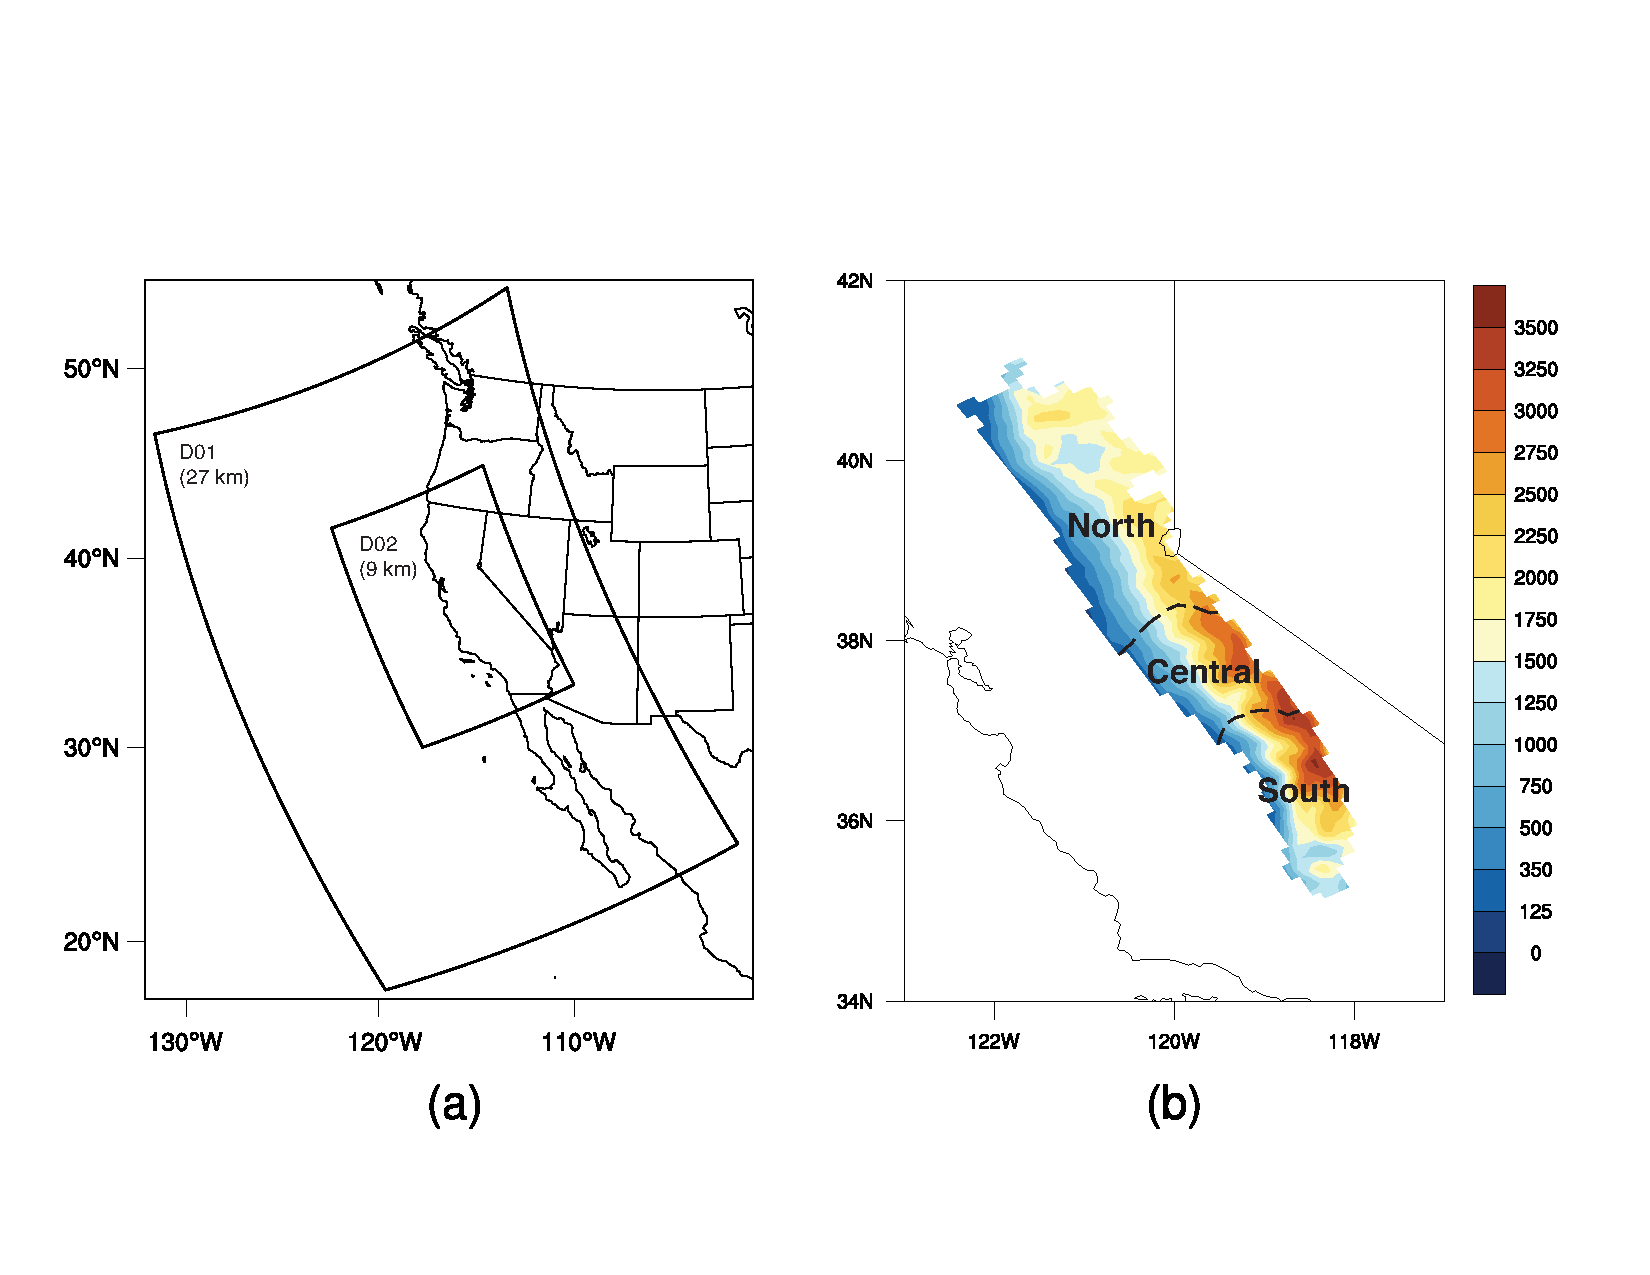
\includegraphics[width=6in]{Fig1.pdf}
\caption{(a) The configuration of WRF at the outer domain (D01, 27 km resolution) and inner domain (D02, 9 km resolution); (b) Topography of the study area covering the Sierra Nevada region within the inner domain (unit: m). Boundaries of the north, central, and south subdivisions are shown by thin black dashed lines.}
\label{fig:wrfdomain}
\end{center}
\end{figure}


%Figure 2: a) changing trend of SWE (without the foothill) b) 2d SWE difference from reference case (drafted) (to be updated) (add y axis label on each side)

\begin{figure}
\begin{center}
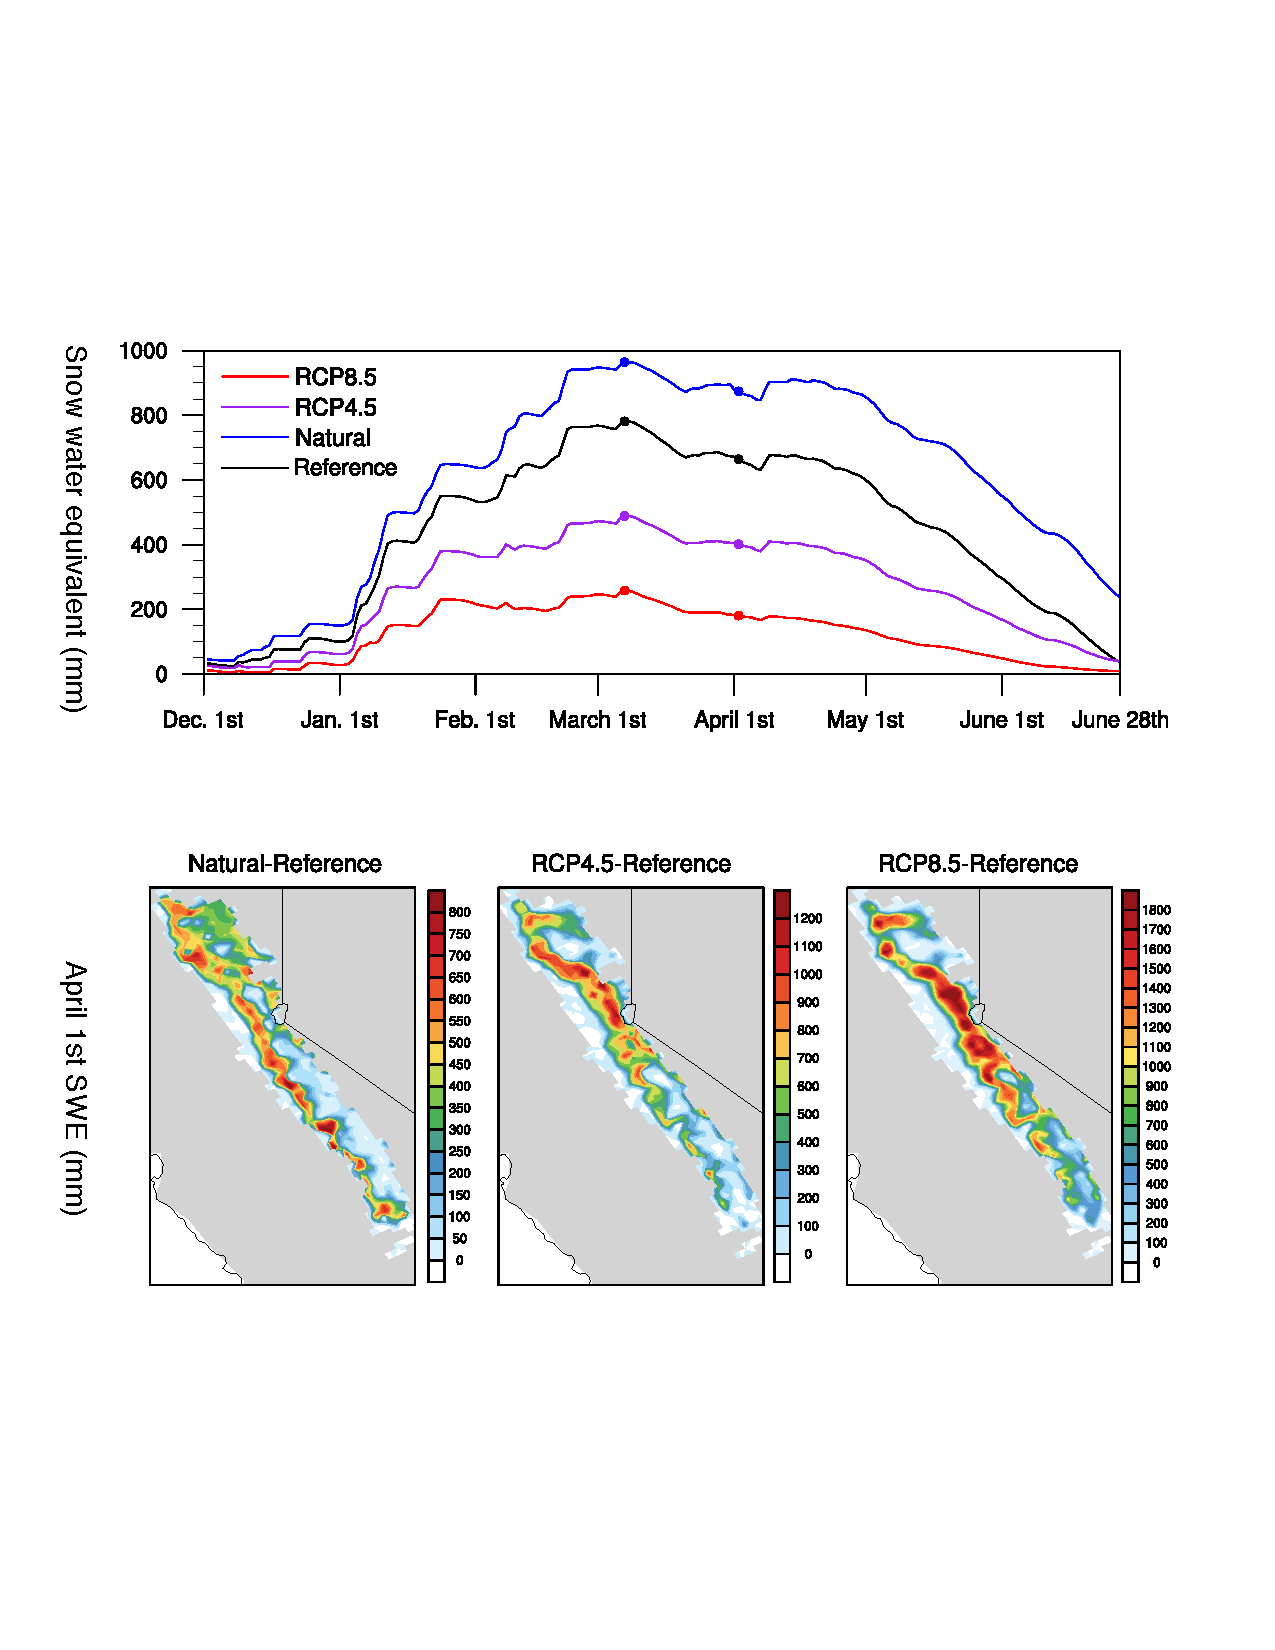
\includegraphics[width=6in, trim={0.2cm 4.5cm 0.2cm 4.0cm},clip]{Fig2.pdf}
\caption{Upper panel: Daily SWE from December 1, 2016 to June 1, 2017 for the reference run (black line), natural (blue), RCP4.5 (purple), and RCP8.5 (red) cases averaged over all grid cells above the foothill area of the Sierra Nevada (note: the maximum and April 1st SWE values are marked with filled dots.); Lower panel: Spatial patterns of differences between the experimental cases and the reference simulation for April 1st SWE of 2017.}
\label{fig:swe}
\end{center}
\end{figure}

%Figure 3: a) the changes of runoff (drafted)

\begin{figure}
\begin{center}
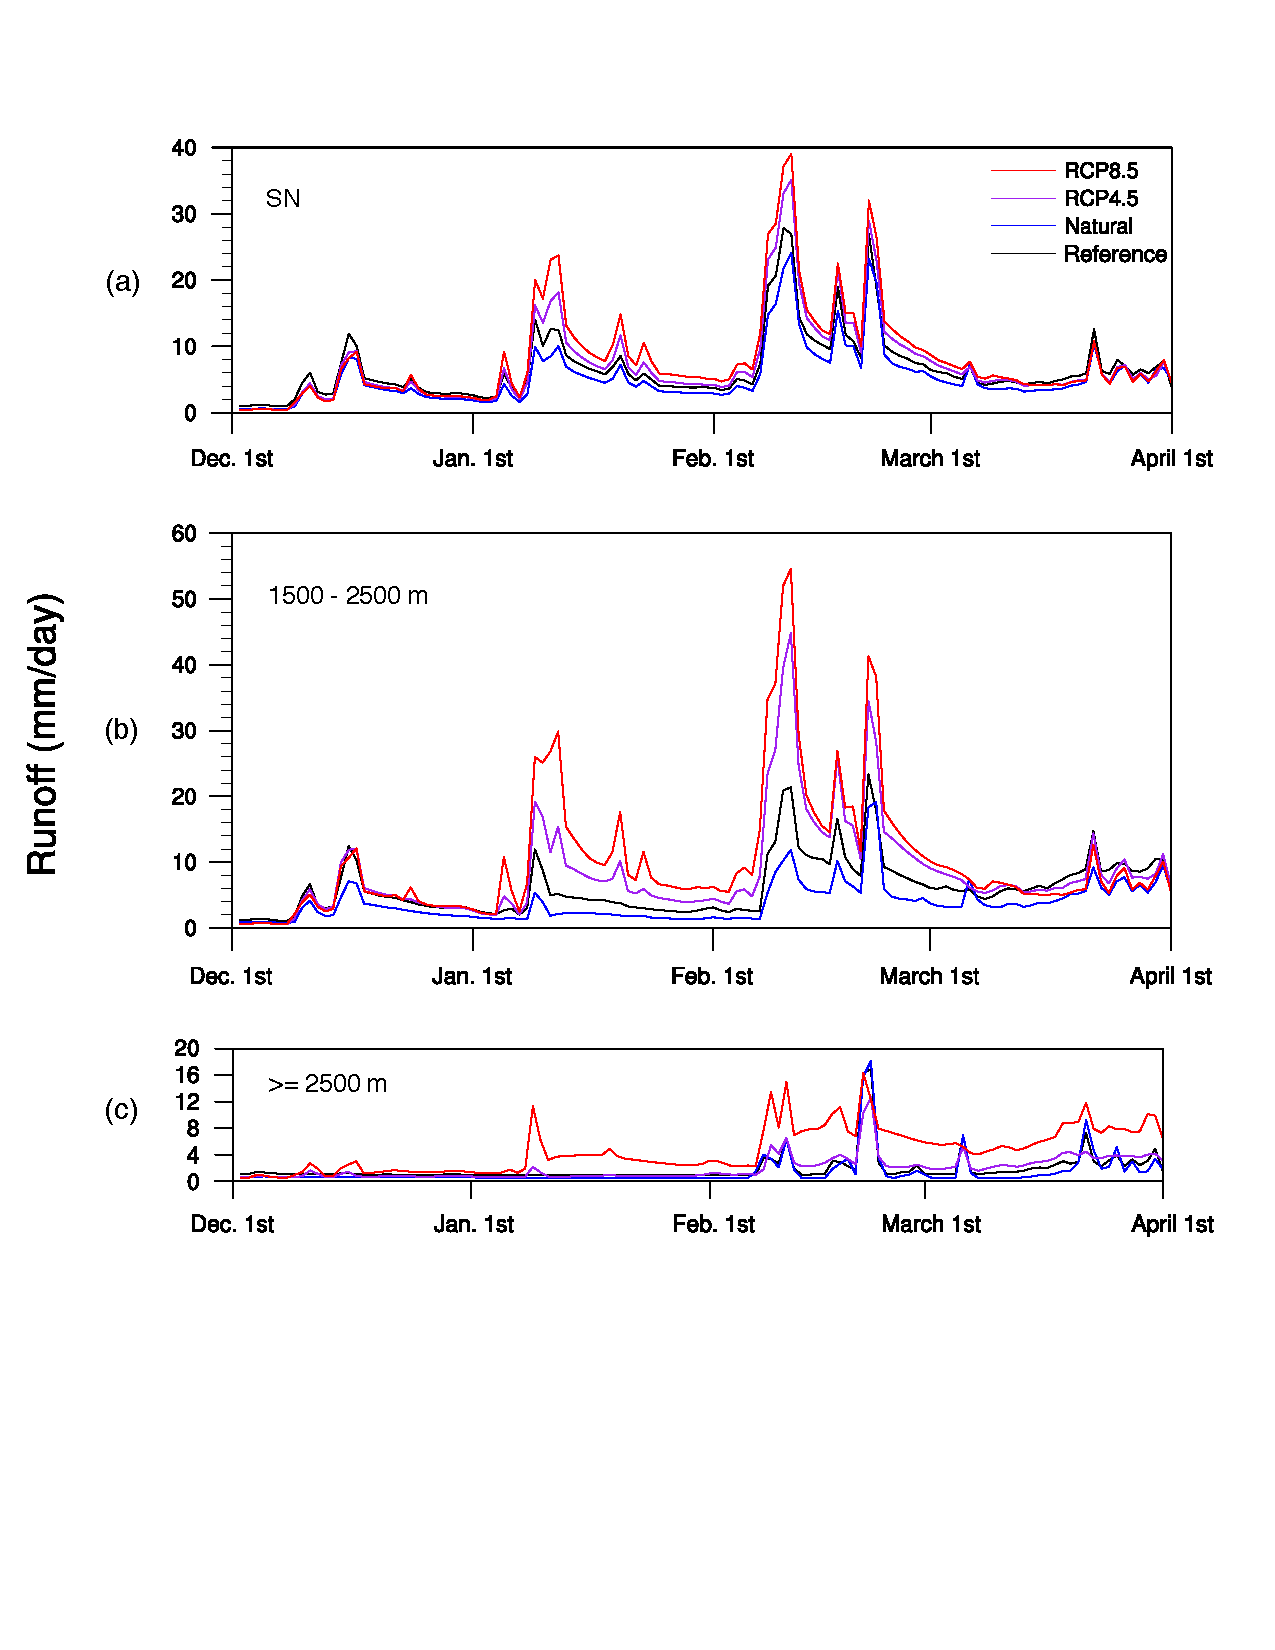
\includegraphics[width=6in]{Fig3.pdf}
\caption{(a) Daily runoff from December 1, 2016 to April 1, 2017 for the reference case (black line), natural (blue), RCP4.5 (purple), and RCP8.5 (red) cases averaged over all of the Sierra Nevada area; (b) Similar as (a), but for the mid-elevation (1500 to 2500 m) regions; (c) Similar as (b), but for the high-elevation areas (above 2500 m).}
\label{fig:runoff}
\end{center}
\end{figure}

%Figure 4: PDF of T2, swe and runoff (drafted) (replot with complete PDF shape) over whole study area with hgt between 1500 to 2500, for year 2017

\begin{figure}
\begin{center}
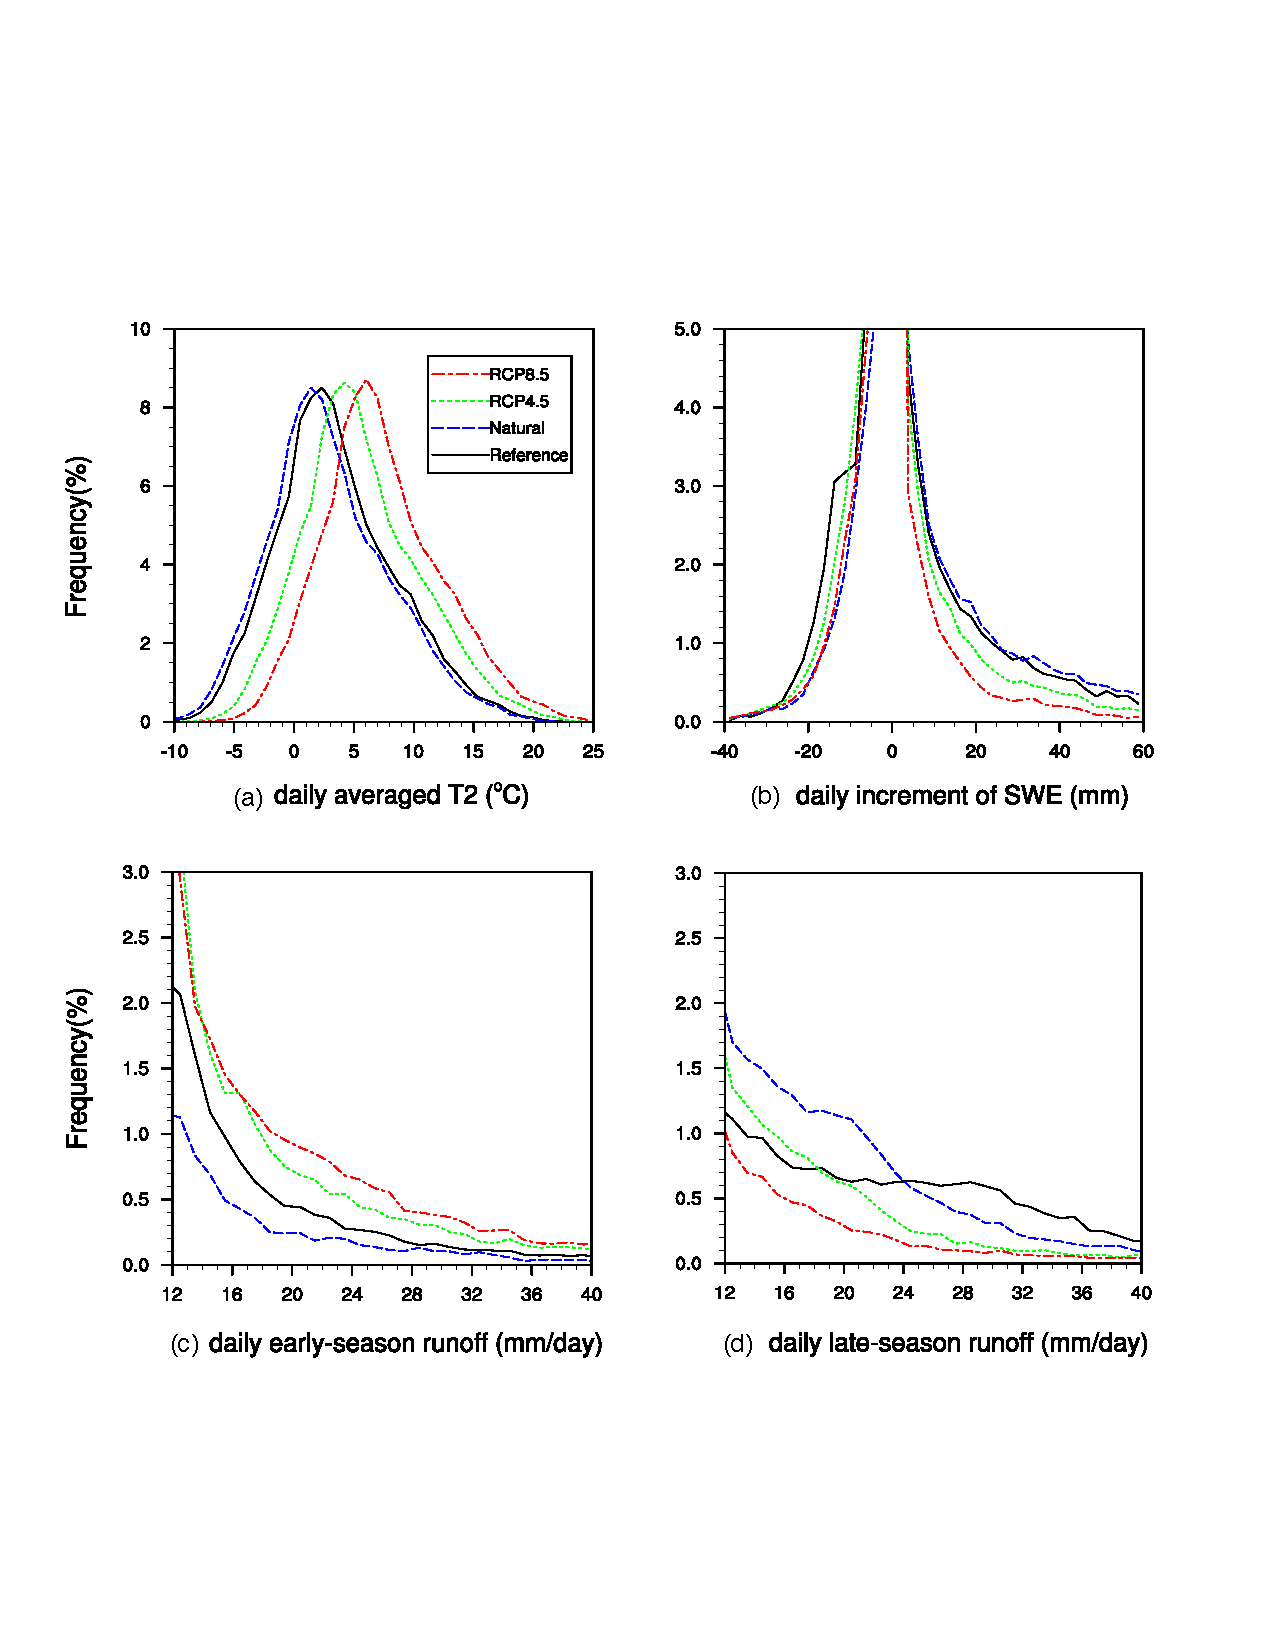
\includegraphics[width=6in]{Fig4.pdf}
\caption{Frequency distributions of daily, mid-elevation (1500 to 2500 m) T2 (a), SWE (b), and early-season runoff (c) for all cases from December 1, 2016 to April 1, 2017. Panel (d): Frequency distribution of daily late-season runoff from April 1 to June 30, 2017 covering mid-elevations and high-elevations.}
\label{fig:pdf}
\end{center}
\end{figure}


%Word limit: Abstract is succinct (<150 words); 12 publication units minus 1 minus 4, i.e. 7*500 = 3500 words excluding the title, authors, affiliations, text in tables (but not captions) and references

\end{document}
